\documentclass{article}
\usepackage{graphicx}
\usepackage{listings}
\usepackage{enumitem}
\usepackage{hyperref}

\title{Design and Implementation of a C-based Spreadsheet Program}
\author{COP290 Project Documentation}
\date{}

\begin{document}
\maketitle

\section{Program Structure and Design Decisions}

\subsection{Modular Architecture}
The program follows a modular design with six core components:
\begin{itemize}
    \item \textbf{Initialization Module (init.c/h)}: Handles memory allocation and sheet initialization
    \item \textbf{I/O Handler (io.c/h)}: Manages input parsing and command validation
    \item \textbf{Process Handler (process.c/h)}: Executes commands and evaluates formulas
    \item \textbf{Display Manager (display.c/h)}: Controls the visual representation
    \item \textbf{Dependency Manager (dependent.c/h)}: Manages cell relationships and updates
    \item \textbf{Stack Operations (stack.c/h)}: Provides auxiliary data structure support.
\end{itemize}

\begin{figure}
        \centering
        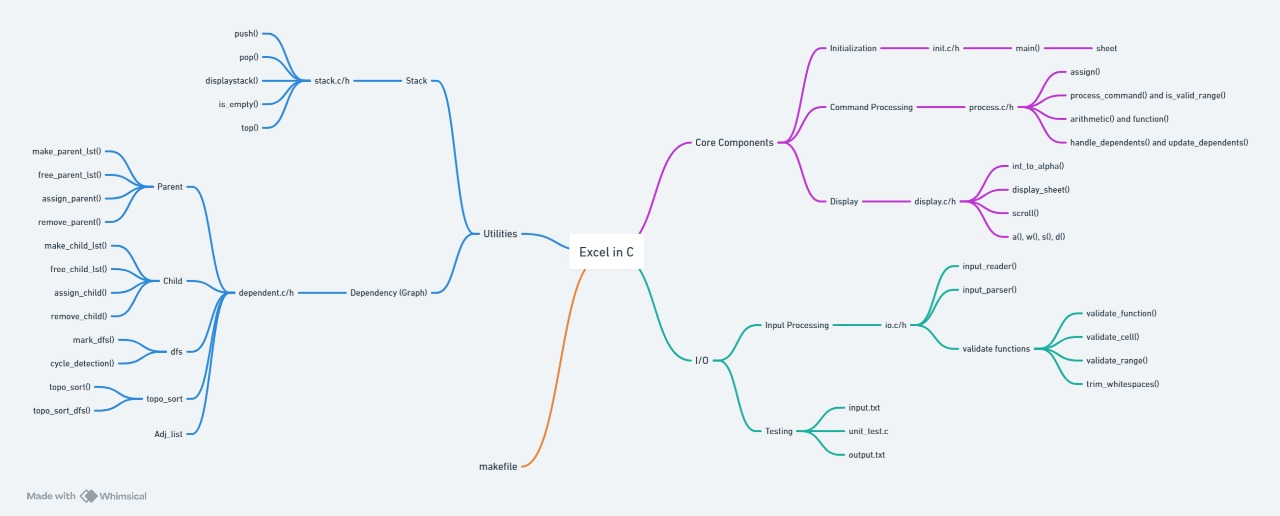
\includegraphics[width=0.9\linewidth]{assets/design.png}
        \label{fig:enter-label}
\end{figure}

\subsection{Key Design Decisions}
\begin{enumerate}
    \item \textbf{Cell Dependencies}
    \begin{itemize}
        \item Implementation of parent-child relationships for formula tracking
        \item Use of adjacency lists for cycle detection
        \item Topological sorting for ordered updates
    \end{itemize}

    \item \textbf{Command Processing}
    \begin{itemize}
        \item Structured parsing using ParsedCommand data structure
        \item Support for arithmetic operations and cell ranges
        \item Implementation of statistical functions (MIN, MAX, SUM, AVG, STDEV)
    \end{itemize}

    \item \textbf{Memory Management}
    \begin{itemize}
        \item Dynamic allocation for sheet structure
        \item Careful memory cleanup to prevent leaks
        \item Efficient storage of formulas and dependencies
    \end{itemize}
\end{enumerate}

\section{Implementation Challenges}

\subsection{Technical Challenges}
\begin{enumerate}
    \item \textbf{Circular Dependency Detection}
    \begin{itemize}
        \item Challenge: Detecting cycles in formula references
        \item Solution: Implementation of depth-first search algorithm
        \item Prevention of infinite loops during cell updates
    \end{itemize}

    \item \textbf{Formula Evaluation}
    \begin{itemize}
        \item Challenge: Parsing and evaluating complex formulas
        \item Solution: Stack-based evaluation system
        \item Handling of nested functions and arithmetic operations
    \end{itemize}

    \item \textbf{Memory Management}
    \begin{itemize}
        \item Challenge: Managing dynamic memory for cells and dependencies
        \item Solution: Structured allocation and deallocation procedures
        \item Prevention of memory leaks in dependency updates
    \end{itemize}
    
    \item \textbf{SLEEP Function}
    \begin{itemize}
        \item Challenge: Implementing time delays without blocking spreadsheet operations
        \item Solution: Custom function type with dependency-aware sleep mechanism
        \item Prevention of deadlocks in formula evaluation chains
    \end{itemize}
\end{enumerate}

\section{Error Handling and Edge Cases}

\subsection{Input Validation}
\begin{itemize}
    \item Cell reference validation (e.g., "A1", "ZZ999")
    \item Formula syntax checking
    \item Range validation (e.g., "A1:B10")
    \item Function name and argument validation
\end{itemize}

\subsection{Error Scenarios Handled}
\begin{enumerate}
    \item \textbf{Formula Errors}
    \begin{itemize}
        \item Division by zero
        \item Invalid cell references
        \item Malformed expressions
        \item Circular dependencies
    \end{itemize}

    \item \textbf{Range Errors}
    \begin{itemize}
        \item Invalid range specifications
        \item Out-of-bounds references
        \item Empty cell ranges in functions
    \end{itemize}

    \item \textbf{Memory Errors}
    \begin{itemize}
        \item Allocation failures
        \item Memory leak prevention
        \item Buffer overflow protection
    \end{itemize}
\end{enumerate}

\section{Test Suite Coverage}

\subsection{Unit Tests (tests)}
\begin{enumerate}
    \item \textbf{Input Parsing Tests}
    \begin{itemize}
        \item Command type identification
        \item Parameter extraction
        \item Formula parsing
        \item Function argument validation
    \end{itemize}

    \item \textbf{Validation Tests}
    \begin{itemize}
        \item Cell reference validation
        \item Range specification validation
        \item Function name validation
        \item Numeric input validation
    \end{itemize}

    \item \textbf{Cell Conversion Tests}
    \begin{itemize}
        \item String to row/column conversion
        \item Boundary value testing
        \item Invalid input handling
    \end{itemize}
\end{enumerate}

\subsection{Edge Case Coverage}
\begin{enumerate}
    \item \textbf{Formula Evaluation}
    \begin{itemize}
        \item Complex nested formulas
        \item Multiple cell references
        \item Statistical function edge cases
        \item Error propagation
    \end{itemize}

    \item \textbf{Dependency Management}
    \begin{itemize}
        \item Circular reference detection
        \item Multiple dependency chains
        \item Update propagation
        \item Dependency cleanup
    \end{itemize}

    \item \textbf{Memory Management}
    \begin{itemize}
        \item Large sheet handling
        \item Dynamic resizing
        \item Resource cleanup
    \end{itemize}
\end{enumerate}

\end{document}
